\begin{quote} \textit{ 4) El regulador se ha diseñado para operar en modo discontinuo con $D<0,5$. Verificar si para $D>0,5$ el regulador pasa a operar en modo continuo. ¿Qué observará en las señales de tensión y corriente de todos o alguno de los componentes para determinar el si el regulador está operando en modo continuo o discontinuo?}
\end{quote}

%\Flor{ Creo que falta algún gráfico, mepa que no pusheaste las simulaciones Nico} 
	Se cambio el valor del ciclo de trabajo a  $ D= 0,8 $ y se obtienen los siguientes resultados

\begin{figure}[H]
	\centering
	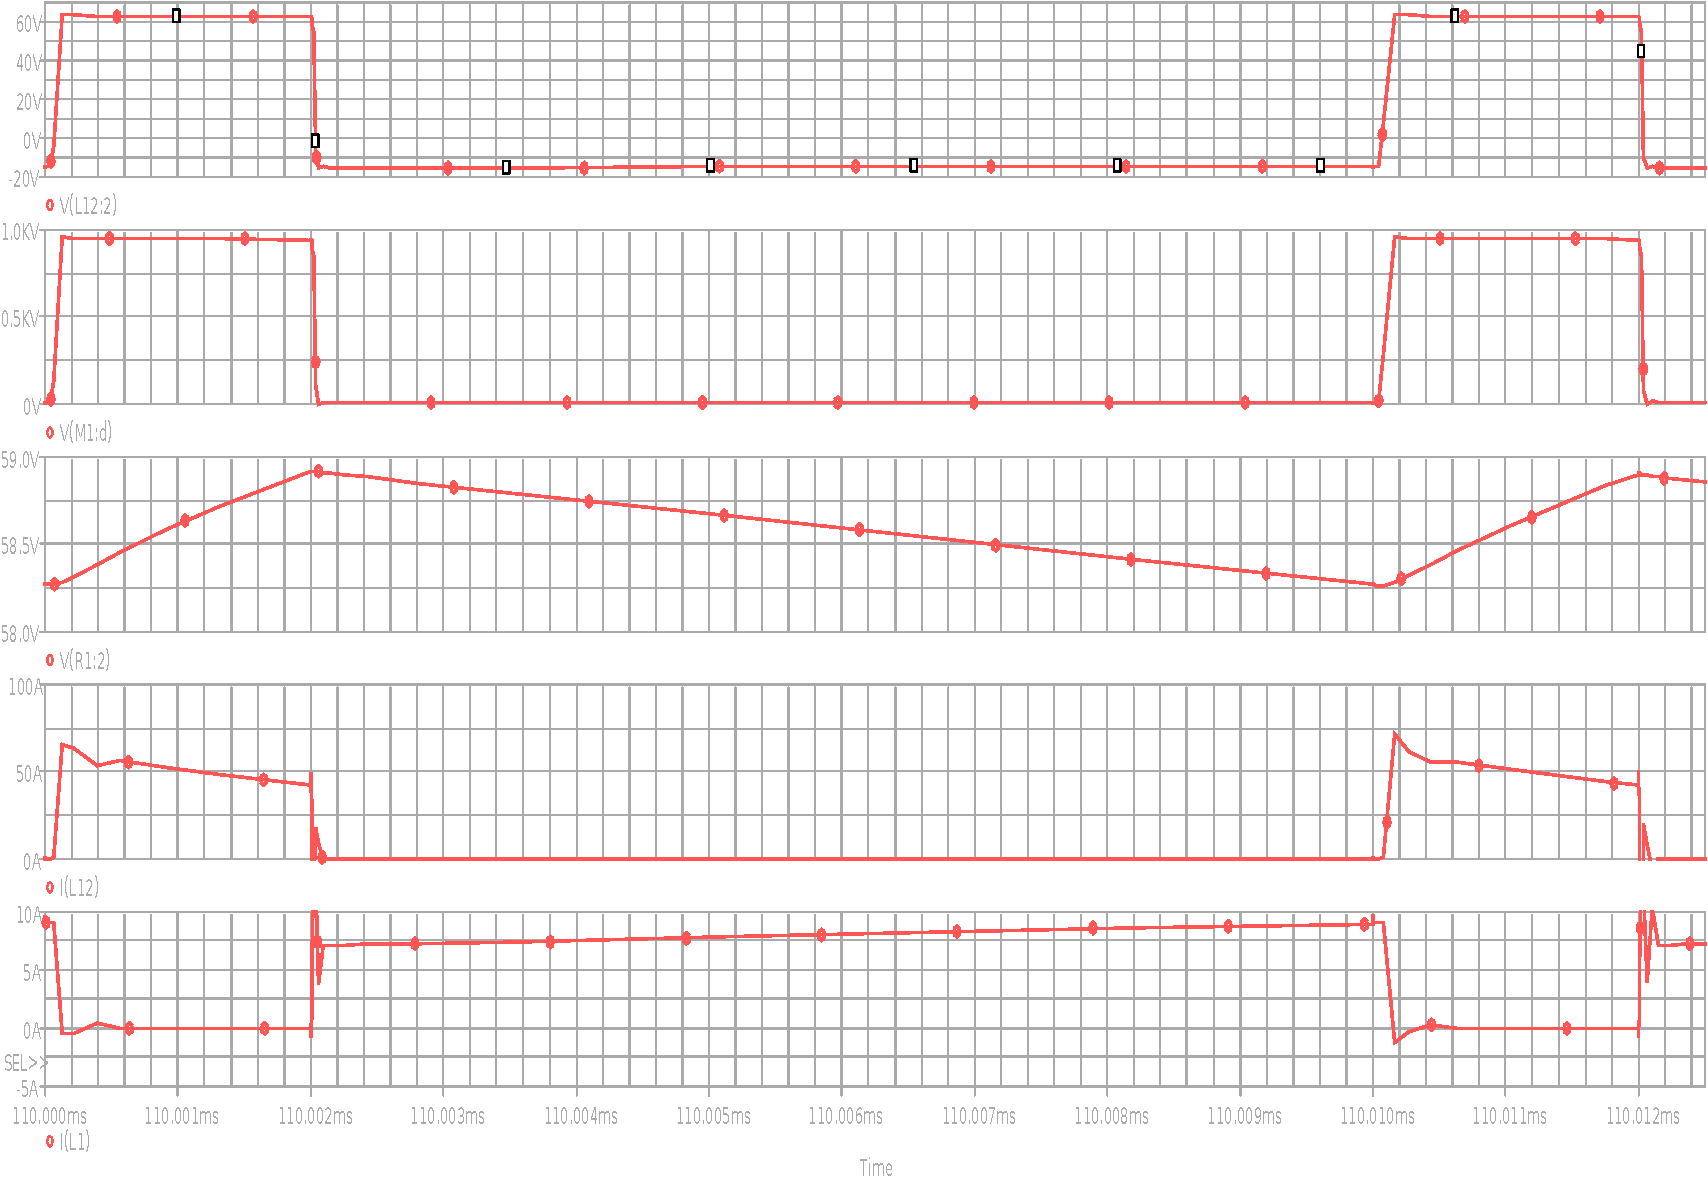
\includegraphics[width=\textwidth]{Figuras/ej4_sim.pdf}
	\caption{Régimen permanente en modo contínuo.}
	\label{fig:permanente_mcc}
\end{figure}

	Como se puede observar en \ref{fig:permanente_mcc} el circuito superado el ciclo de trabajo máximo pasa a operar en modo contínuo, ya que la corriente en el inductor no se interrumpe en todo el ciclo de trabajo. 
	\indent En el caso de que se quiera seguir operando en modo discontínuo para dicho ciclo de trabajo se deberia utilizar los siguientes valores de inducciones. 

\begin{align*}
	\centering
	& I_{max} = \frac{ 2 \cdot \SI{36.4}{\watt} }{\SI{150}{\volt} \cdot \num{0,8}} = \SI{0.61}{\ampere} \\
	& L_{1,max} = \frac{\SI{150}{\volt} \cdot \num{0,8}}{\SI{0.61}{\ampere} \SI{100}{\kilo\ohm}} \simeq \SI{1.97}{\milli\henry} \\
	& N_{12} = \frac{ (12+1)(1-0,8) \cdot N_1}{ (150-2) \cdot 0,8} = \frac{13 \cdot N_1}{592} \implies \boxed{L_{12} \simeq \SI{0.95}{\micro\henry}} \\
	& N_5 = \frac{(5+1)(1-0,8) \cdot N_1}{(150-2) \cdot 0,8} = \frac{3 \cdot N_1}{296} \implies \boxed{L_5 \simeq \SI{0.2}{\micro\henry}}
\end{align*}


%\begin{itemize}
%	\item Modo continuo:\hspace{0.4cm} $ \frac{1}{2} \Delta I_L < I_o $
%	\item Modo discontinuo: $ \frac{1}{2} \Delta I_L > I_o $
%\end{itemize}


%\begin{align*}
%	\centering
%	D_{max} &= 0,5 \implies \frac{1}{2} \cdot \SI{20}{\ampere} > I_o = \SI{2}{\ampere} \\
%	D_{max} &= 0,8 \implies \frac{1}{2} \cdot \SI{7.5}{\ampere} > I_o = \SI{2}{\ampere}
%\end{align*}
